
%%%%%%%%%%

\begin{frame}{\vskip -0.2cm\Large Premier achat document\'e d'un objet physique gr\^ace \`a des bitcoins}

\begin{multicols}{2}

	\begin{flushleft}
	\mbox{}\vskip -0.4cm
	%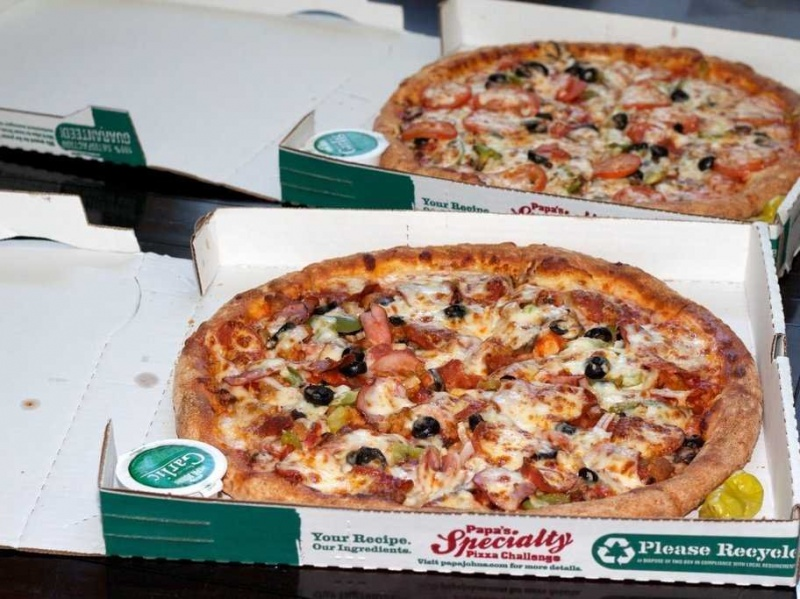
\includegraphics[width=12cm]{graphics/800px-Laszlospizza.jpg}
	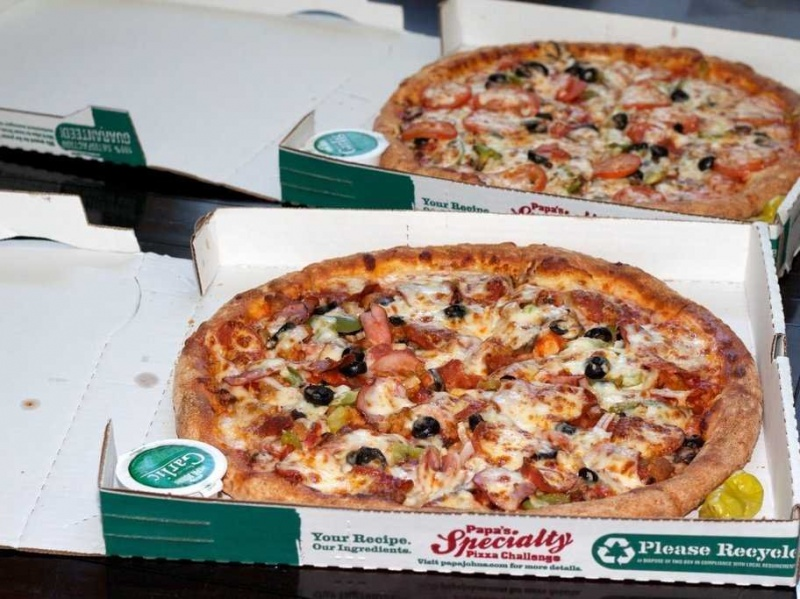
\includegraphics[height=5.5cm]{graphics/800px-Laszlospizza.jpg}
	\vskip -0.1cm
	{\tiny\texttt{https://en.bitcoin.it/wiki/Laszlo\_Hanyecz}}
	\vskip -0.2cm
	{\tiny\texttt{https://bitcointalk.org/index.php?topic=137.msg1195\#msg1195}}
	
	\end{flushleft}

\columnbreak

	\begin{flushright}

		\begin{minipage}{2.7cm}{\bf
		\begin{center}
		
		\mbox{}\vskip 0.2cm
		{\huge\color{red}2 pizzas}
		\vskip 0.5cm
		{\Large 10,000 BTC}
		\vskip 0.5cm
		{\Large 22 mai 2010}
		\vskip -0.175cm
		{\tiny(Journ\'ee de Pizza Bitcoin)}		
		\vskip 0.5cm
		Laszlo Hanyecz
		\vskip -0.1cm
		{\tiny\begin{itemize}
		\item
			un des premiers mineurs de bitcoin
		\item
			d\'eveloppeur informatique am\'ericain
		\end{itemize}}
				
		\end{center}
    		}\end{minipage}
		
	
	\end{flushright}

\end{multicols}

\normalsize
\end{frame}

%%%%%%%%%%
